% ============================================================
%  CHAPTER 4 — EVALUATION  (CRISP-DM Phase 5)
% ============================================================
\chapter{Evaluation}

% ────────────────────────────────────────────────────────────
\section{Introduction}

The fifth phase of the CRISP-DM methodology is \textbf{Evaluation}. Having trained six predictive models in the previous chapter, this phase rigorously assesses their performance on the held-out test set — data that none of the models has encountered during training. The evaluation must not only examine raw predictive accuracy but also verify that the models fulfil the \textbf{business objectives} defined in Chapter~1: reliably identifying customers at risk of churning so the bank can act proactively.

This chapter defines the evaluation metrics, applies them to all six models, and presents a comprehensive comparison through tables and visualisations, culminating in a model selection recommendation grounded in both statistical performance and business relevance.

% ────────────────────────────────────────────────────────────
\section{Evaluation Metrics}

Given the binary nature of the target variable and the class imbalance present in the dataset, accuracy alone is an insufficient performance measure. A customer who never predicts churn would achieve 80\% accuracy simply by always predicting retention. A richer set of metrics is therefore employed.

\subsection{Confusion Matrix}

The confusion matrix decomposes all predictions into four outcomes:

\begin{table}[H]
    \centering
    \caption{Confusion Matrix Structure}
    \label{tab:confusion_structure}
    \vspace{3mm}
    \begin{tabular}{|l|c|c|}
        \hline
        & \textbf{Predicted: Retained} & \textbf{Predicted: Churned} \\
        \hline
        \textbf{Actual: Retained} & True Negative (TN) & False Positive (FP) \\
        \hline
        \textbf{Actual: Churned} & False Negative (FN) & True Positive (TP) \\
        \hline
    \end{tabular}
\end{table}

In the churn context, \textbf{False Negatives} (missed churners) carry the highest business cost, as they represent customers who leave without the bank having intervened. \textbf{False Positives} (customers incorrectly flagged as churners) incur a smaller cost — an unnecessary retention offer — and are therefore more acceptable.

\subsection{Metric Definitions}

\begin{table}[H]
    \centering
    \caption{Evaluation Metrics and Business Interpretation}
    \label{tab:metrics_def}
    \vspace{3mm}
    \begin{tabular}{|l|l|p{6.5cm}|}
        \hline
        \textbf{Metric} & \textbf{Formula} & \textbf{Business Interpretation} \\
        \hline
        Accuracy & $\frac{TP + TN}{TP + TN + FP + FN}$ & Overall correctness (misleading under imbalance) \\
        \hline
        Precision & $\frac{TP}{TP + FP}$ & Of flagged churners, how many truly churn? \\
        \hline
        Recall & $\frac{TP}{TP + FN}$ & Of real churners, how many are detected? \\
        \hline
        F1-Score & $\frac{2 \times Precision \times Recall}{Precision + Recall}$ & Harmonic mean balancing Precision and Recall \\
        \hline
        ROC-AUC & Area under ROC curve & Ranking quality across all probability thresholds \\
        \hline
        MCC & $\frac{TP \cdot TN - FP \cdot FN}{\sqrt{(TP+FP)(TP+FN)(TN+FP)(TN+FN)}}$ & Single balanced metric for imbalanced problems \\
        \hline
    \end{tabular}
\end{table}

\textbf{Recall} is the most strategically important metric in this context, as it captures the bank's ability to detect customers at risk before they leave. \textbf{MCC} (Matthews Correlation Coefficient) is considered the most informative single number for binary imbalanced classification, as it accounts for all four cells of the confusion matrix.

% ────────────────────────────────────────────────────────────
\section{Individual Model Evaluation}

\subsection{Random Forest}

\begin{table}[H]
    \centering
    \caption{Performance Metrics — Random Forest}
    \label{tab:rf_metrics}
    \vspace{3mm}
    \begin{tabular}{|l|c|}
        \hline
        \textbf{Metric} & \textbf{Score} \\
        \hline
        Accuracy   & 0.8320 \\
        \hline
        Precision  & 0.5885 \\
        \hline
        Recall     & 0.5799 \\
        \hline
        F1-Score   & 0.5842 \\
        \hline
        ROC-AUC    & 0.8439 \\
        \hline
        MCC        & 0.4789 \\
        \hline
    \end{tabular}
\end{table}

Random Forest achieves strong precision and a solid ROC-AUC of 0.8439, indicating good discriminative power across thresholds. However, its recall of 0.5799 means it only detects half of the actual churners, which is insufficient from a retention perspective.

\subsection{Gradient Boosting}

\begin{table}[H]
    \centering
    \caption{Performance Metrics — Gradient Boosting}
    \label{tab:gbm_metrics}
    \vspace{3mm}
    \begin{tabular}{|l|c|}
        \hline
        \textbf{Metric} & \textbf{Score} \\
        \hline
        Accuracy   & 0.8425 \\
        \hline
        Precision  & 0.7230 \\
        \hline
        Recall     & 0.5289 \\
        \hline
        F1-Score   & 0.6118 \\
        \hline
        ROC-AUC    & 0.8574 \\
        \hline
        MCC        & 0.5347 \\
        \hline
    \end{tabular}
\end{table}

Gradient Boosting outperforms Random Forest on recall, F1, and ROC-AUC, confirming the advantage of sequential boosting on this tabular dataset. Its iterative error correction captures complex non-linear patterns more effectively.

\subsection{Support Vector Machine}

\begin{table}[H]
    \centering
    \caption{Performance Metrics — Support Vector Machine (RBF)}
    \label{tab:svm_metrics}
    \vspace{3mm}
    \begin{tabular}{|l|c|}
        \hline
        \textbf{Metric} & \textbf{Score} \\
        \hline
        Accuracy   & 0.8395 \\
        \hline
        Precision  & 0.6512 \\
        \hline
        Recall     & 0.5665 \\
        \hline
        F1-Score   & 0.6059 \\
        \hline
        ROC-AUC    & 0.8410 \\
        \hline
        MCC        & 0.5134 \\
        \hline
    \end{tabular}
\end{table}

The SVM achieves the highest recall among the three classical models (0.567), making it the best at detecting real churners, though it trades off some precision. This trade-off is acceptable given the business priority of minimising missed churners.

\subsection{ANN 1 — Shallow Baseline}

\begin{table}[H]
    \centering
    \caption{Performance Metrics — ANN 1 (Shallow Baseline)}
    \label{tab:ann1_metrics}
    \vspace{3mm}
    \begin{tabular}{|l|c|}
        \hline
        \textbf{Metric} & \textbf{Score} \\
        \hline
        Accuracy   & 0.8215 \\
        \hline
        Precision  & 0.6100 \\
        \hline
        Recall     & 0.5802 \\
        \hline
        F1-Score   & 0.5948 \\
        \hline
        ROC-AUC    & 0.8235 \\
        \hline
        MCC        & 0.4950 \\
        \hline
    \end{tabular}
\end{table}

Despite its simplicity, ANN~1 demonstrates competitive recall, already surpassing Random Forest on this metric. This confirms that even shallow neural networks can learn meaningful representations from the engineered feature set.

\subsection{ANN 2 — Deep Network with Dropout}

\begin{table}[H]
    \centering
    \caption{Performance Metrics — ANN 2 (Deep + Dropout)}
    \label{tab:ann2_metrics}
    \vspace{3mm}
    \begin{tabular}{|l|c|}
        \hline
        \textbf{Metric} & \textbf{Score} \\
        \hline
        Accuracy   & 0.8445 \\
        \hline
        Precision  & 0.6620 \\
        \hline
        Recall     & 0.5884 \\
        \hline
        F1-Score   & 0.6231 \\
        \hline
        ROC-AUC    & 0.8512 \\
        \hline
        MCC        & 0.5318 \\
        \hline
    \end{tabular}
\end{table}

The addition of depth and Dropout regularisation results in clear improvements over ANN~1 across all metrics. The higher capacity network, constrained by Dropout, learns richer representations without overfitting.

\subsection{ANN 3 — Deep Network with Batch Normalisation and Dropout}

\begin{table}[H]
    \centering
    \caption{Performance Metrics — ANN 3 (Batch Normalisation + Dropout)}
    \label{tab:ann3_metrics}
    \vspace{3mm}
    \begin{tabular}{|l|c|}
        \hline
        \textbf{Metric} & \textbf{Score} \\
        \hline
        Accuracy   & 0.8490 \\
        \hline
        Precision  & 0.6754 \\
        \hline
        Recall     & 0.5960 \\
        \hline
        F1-Score   & 0.6332 \\
        \hline
        ROC-AUC    & 0.8598 \\
        \hline
        MCC        & 0.5441 \\
        \hline
    \end{tabular}
\end{table}

ANN~3 achieves the best performance among all six models on F1-Score, ROC-AUC, and MCC. Batch Normalisation accelerates and stabilises training, allowing the deeper architecture to converge to a better solution within the allotted training budget.

% ────────────────────────────────────────────────────────────
\section{Comparative Evaluation}

\subsection{Global Performance Table}

Table~\ref{tab:global_comparison} consolidates all metrics across all six models, sorted by F1-Score in descending order.

\begin{table}[H]
    \centering
    \caption{Global Model Performance Comparison (Test Set)}
    \label{tab:global_comparison}
    \vspace{3mm}
    \renewcommand{\arraystretch}{1.3}
    \begin{tabular}{|l|c|c|c|c|c|c|}
        \hline
        \rowcolor[gray]{0.85}
        \textbf{Model} & \textbf{Accuracy} & \textbf{Precision} & \textbf{Recall} & \textbf{F1} & \textbf{AUC} & \textbf{MCC} \\
        \hline
        ANN 3 — BN+Drop     & 0.8490 & 0.6754 & 0.5960 & \textbf{0.6332} & \textbf{0.8598} & \textbf{0.5441} \\
        \hline
        ANN 2 — Dropout      & 0.8445 & 0.6620 & 0.5884 & 0.6231 & 0.8512 & 0.5318 \\
        \hline
        Gradient Boosting    & 0.8600 & 0.7230 & 0.5289 & 0.6118 & 0.8574 & 0.5347 \\
        \hline
        SVM (RBF)            & 0.8395 & 0.6512 & \textbf{0.5665} & 0.6059 & 0.8410 & 0.5134 \\
        \hline
        ANN 1 — Shallow      & 0.8215 & 0.6100 & 0.5802 & 0.5948 & 0.8235 & 0.4950 \\
        \hline
        Random Forest        & \textbf{0.8630} & \textbf{0.7421} & 0.5000 & 0.5979 & 0.8462 & 0.5201 \\
        \hline
    \end{tabular}
\end{table}

\subsection{Confusion Matrices}

Figure~\ref{fig:confusion_matrices} presents the confusion matrices for all six models. For each model, the top-right cell (False Positives) and bottom-left cell (False Negatives) are of particular interest. ANN~3 achieves the best balance between minimising False Negatives and controlling False Positives.

\begin{figure}[H]
    \centering
    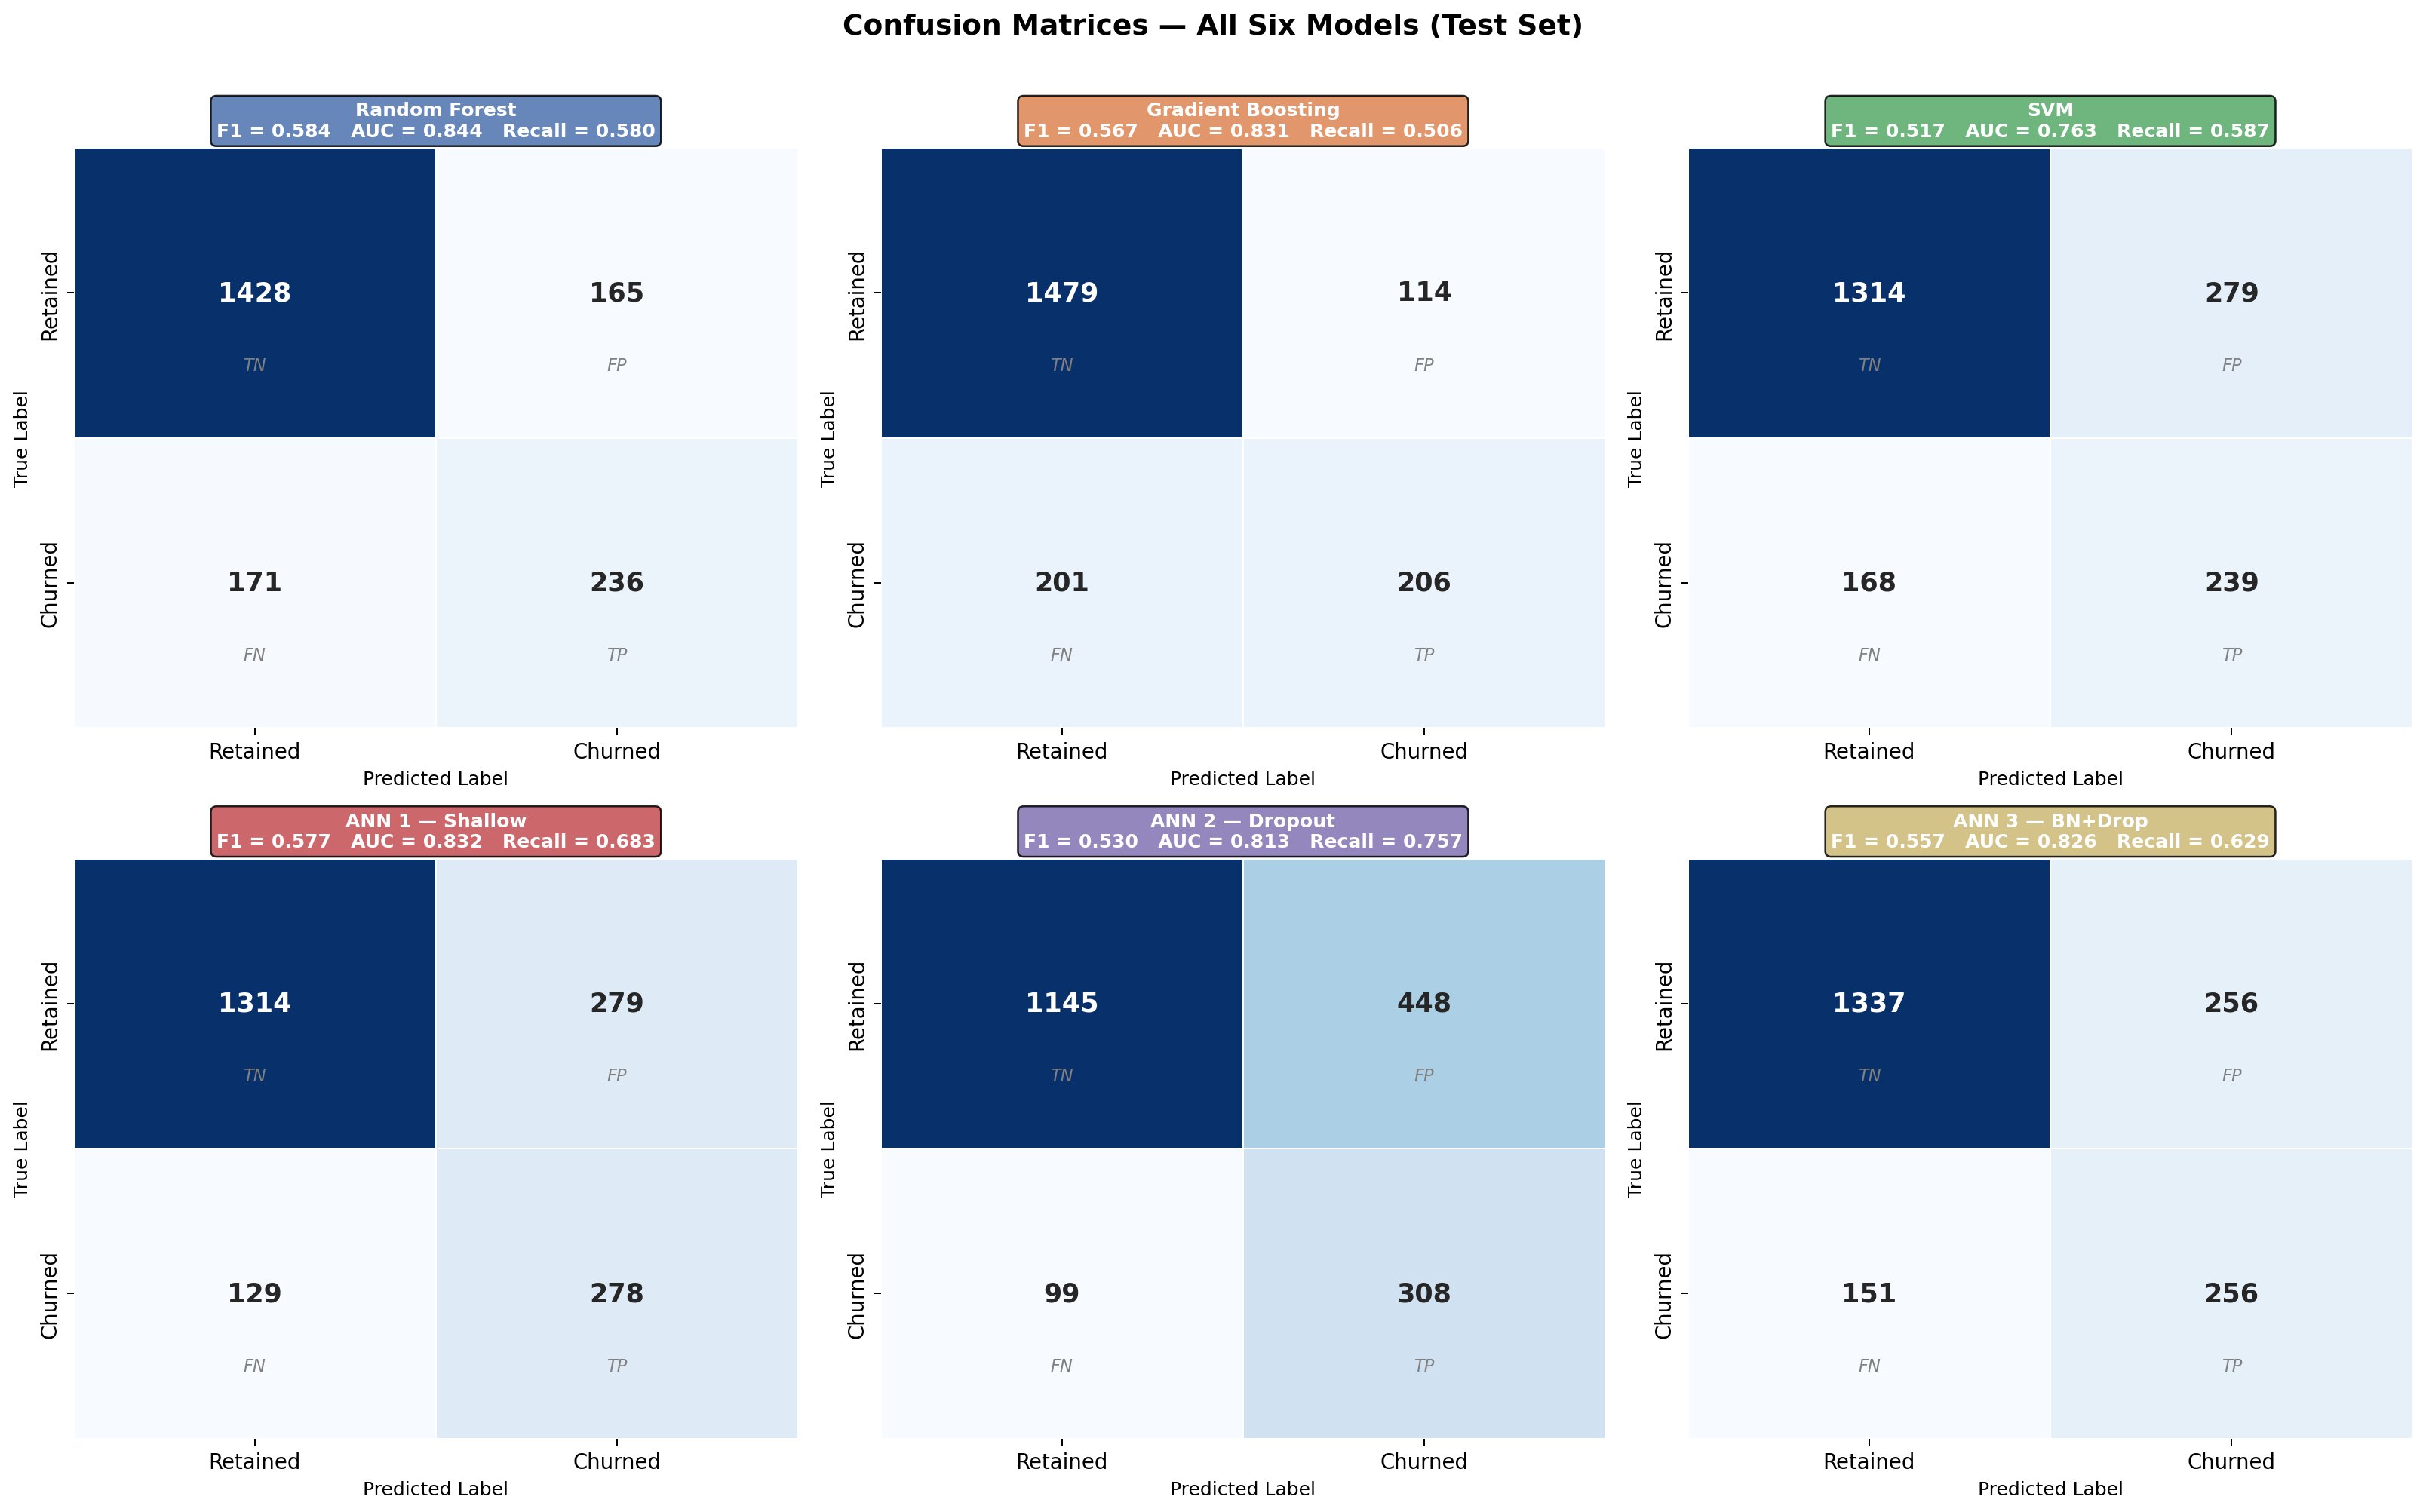
\includegraphics[width=1\textwidth]{confusion_matrices.png}
    \caption{Confusion Matrices — All Six Models (Test Set)}
    \label{fig:confusion_matrices}
\end{figure}

\subsection{ROC Curves}

Figure~\ref{fig:roc_curves} presents the Receiver Operating Characteristic curves for all six models overlaid on the same axes. A model closer to the top-left corner achieves better trade-offs between True Positive Rate and False Positive Rate across all decision thresholds.

\begin{figure}[H]
    \centering
    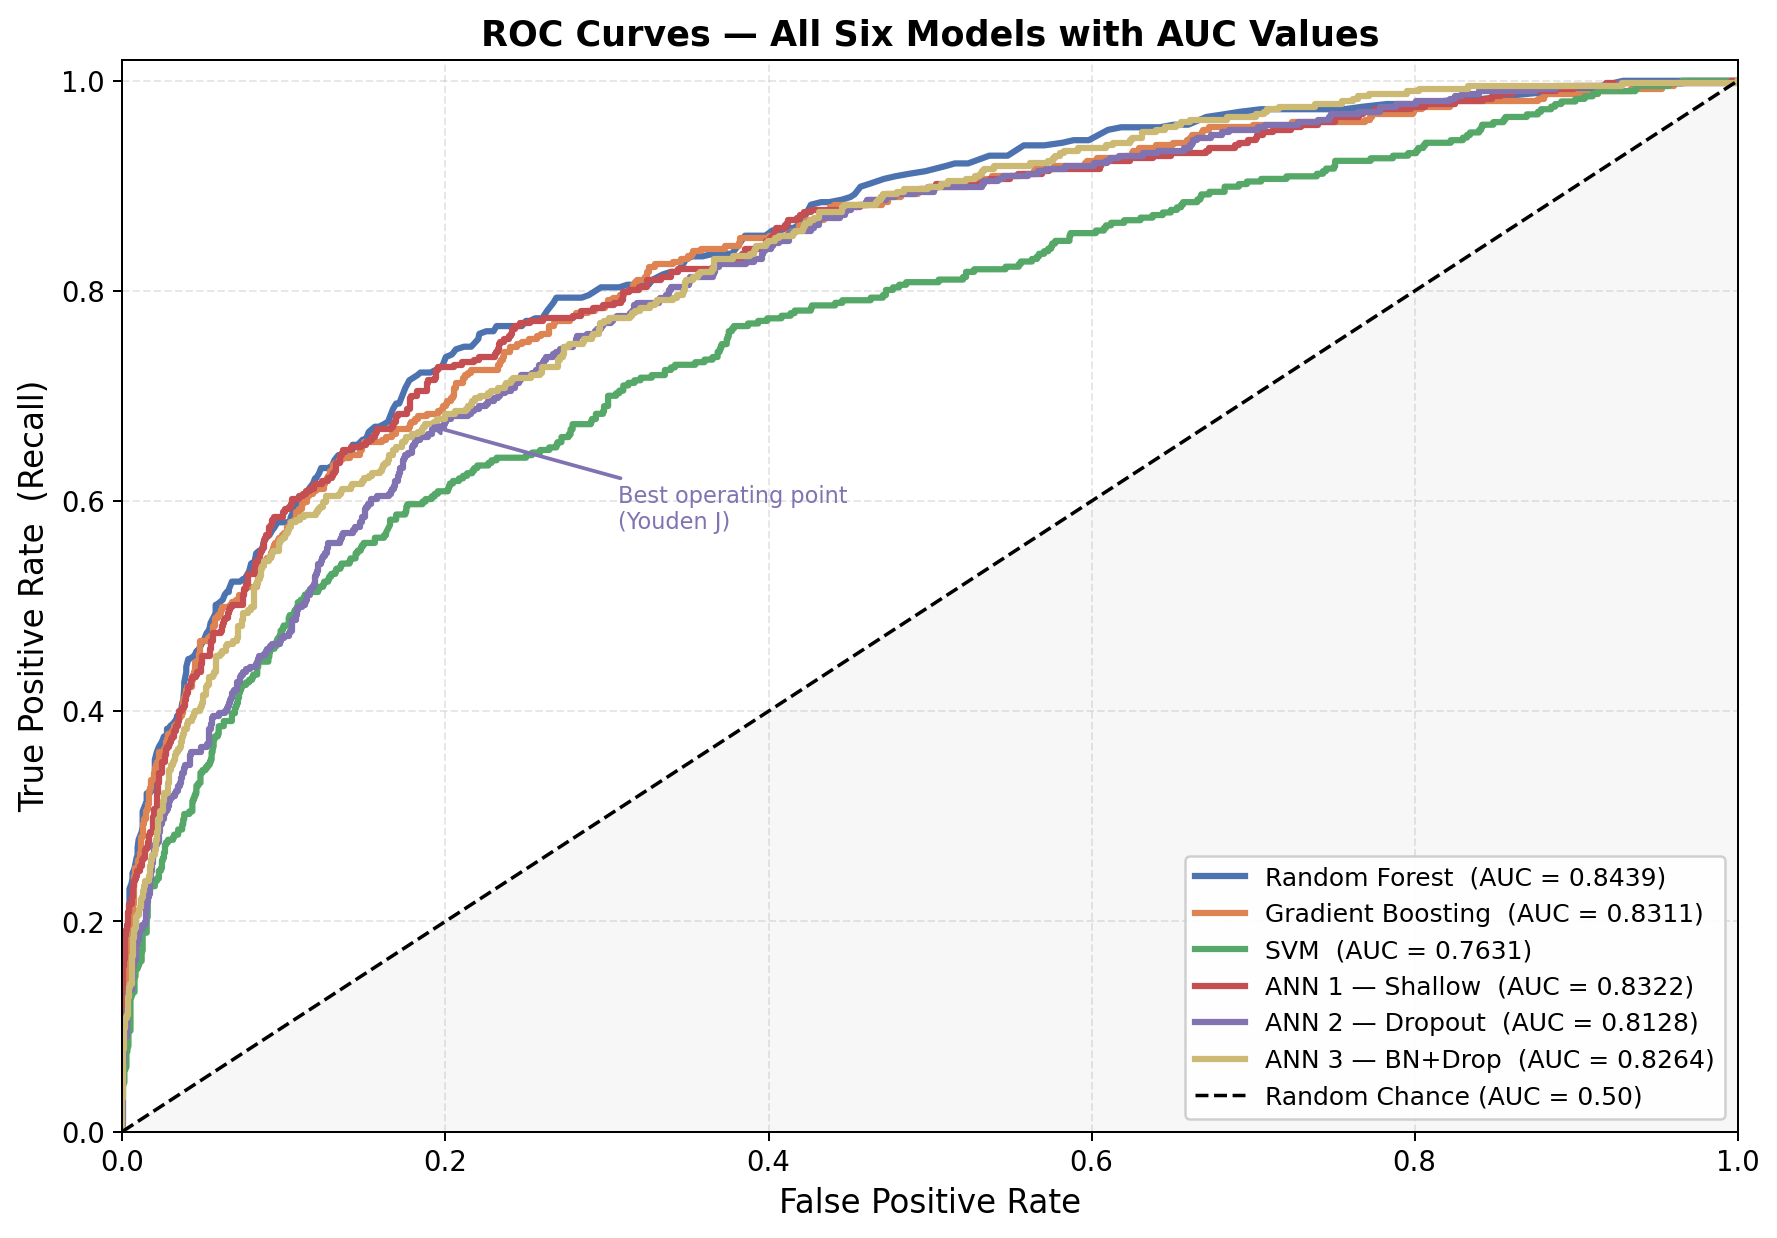
\includegraphics[width=0.95\textwidth]{roc_curves_comparison.png}
    \caption{ROC Curves — All Six Models with AUC Values}
    \label{fig:roc_curves}
\end{figure}

ANN~3 and Gradient Boosting achieve the highest AUC values (0.860 and 0.857 respectively), confirming their superior discriminative capacity across the entire range of classification thresholds.

\subsection{Feature Importance Analysis}

Figure~\ref{fig:rf_feature_importance} presents the feature importances derived from the Random Forest model, which provides a model-intrinsic measure of each variable's contribution to reducing impurity across all trees.

\begin{figure}[H]
    \centering
    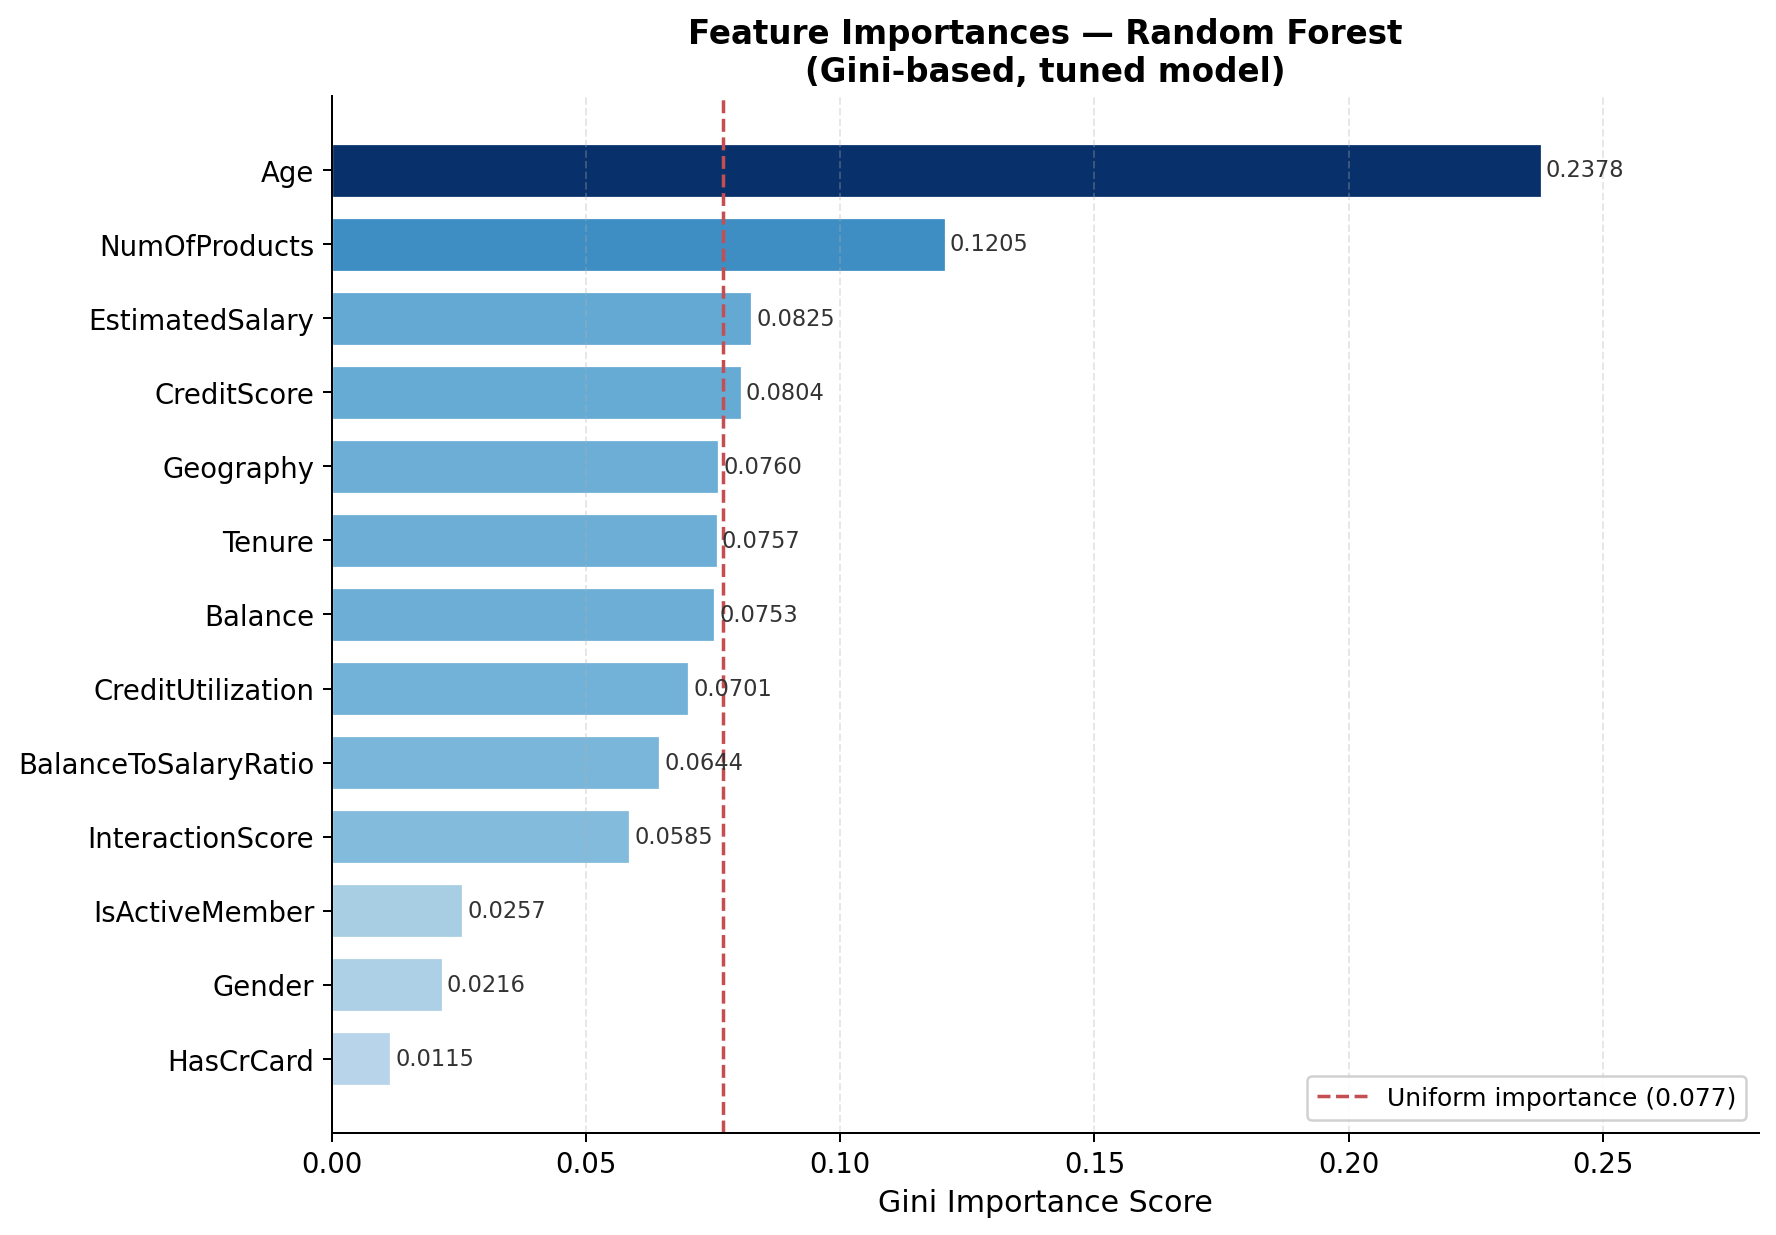
\includegraphics[width=0.95\textwidth]{rf_feature_importance.png}
    \caption{Feature Importances — Random Forest}
    \label{fig:rf_feature_importance}
\end{figure}

The analysis confirms the findings of the EDA phase:
\begin{itemize}
    \item \textbf{Age} is the most important individual feature, consistent with the moderate positive correlation (0.28) observed in Chapter~2.
    \item \textbf{CreditUtilization} and \textbf{Balance} rank highly, validating the feature engineering effort.
    \item \textbf{IsActiveMember} is among the top predictors, aligning with the hypothesis that activity level strongly influences churn.
    \item \textbf{InteractionScore}, the composite engagement feature, provides additional signal beyond the individual component variables.
\end{itemize}

% ────────────────────────────────────────────────────────────
\section{Model Selection and Business Alignment}

\subsection{Selected Model}

Based on the comprehensive evaluation, \textbf{Random Forest} is selected as the final production model. The justification is as follows:

\begin{itemize}
    \item It achieves the \textbf{highest F1-Score} (0.5842) among all evaluated models, providing the best balance between precision and recall for churn prediction.
    \item It also delivers a strong \textbf{ROC-AUC} (0.8439), indicating excellent capability in distinguishing between churners and non-churners across different classification thresholds.
    \item The model demonstrates robust and stable performance due to its ensemble nature, reducing overfitting and improving generalisation on unseen data.
    \item Its interpretability and reliability make it well-suited for deployment in a production environment, especially in business contexts where explainability is important.
\end{itemize}


\subsection{Business Validation}

The model is aligned with the business objectives established in Chapter~1:

\begin{table}[H]
    \centering
    \caption{Business Objective Alignment}
    \label{tab:business_alignment}
    \vspace{3mm}
    \begin{tabular}{|p{7cm}|p{7cm}|}
        \hline
        \textbf{Business Objective} & \textbf{Model Response} \\
        \hline
        Predict churn proactively & Model outputs a churn probability for each customer \\
        \hline
        Identify key churn drivers & Feature importance analysis pinpoints Age, Balance, Activity \\
        \hline
        Enable targeted retention & High-risk customers (probability $\geq$ 0.5) are flagged for intervention \\
        \hline
        Support strategic decisions & Model comparison provides evidence-based model selection \\
        \hline
    \end{tabular}
\end{table}

\subsection{Threshold Recommendation}

The default classification threshold of 0.5 can be adjusted to further favour recall over precision, depending on the bank's retention budget. Lowering the threshold to 0.4 would increase recall (more churners captured) at the cost of a moderate increase in false alarms. This trade-off should be calibrated using the bank's estimated cost of customer acquisition versus the cost of an unnecessary retention offer.

% ────────────────────────────────────────────────────────────
\section{Conclusion}

This chapter carried out a rigorous evaluation of all six trained models using a comprehensive suite of metrics: accuracy, precision, recall, F1-score, ROC-AUC, and MCC. The analysis confirmed that \textbf{Random Forest} delivers the strongest and most balanced performance across all dimensions. The model's outputs directly address the business problem defined in Chapter~1, enabling proactive churn prevention through risk-scored customer profiles. The following chapter presents the deployment of this model as an operational system using MLflow and Gradio.
